\chapter{Конструкторская часть}

По построенной ER диаграмме, можно выделить следующие сущности БД:

\section{Требования к программному обеспечению}

Разрабатываемое программное обеспечение должно предоставлять
следующие функциональные возможности:

\begin{itemize}
  \item генерация случайного графа заданной плотности;
  \item сохранение графа в базу данных;
  \item выполнение алгоритма Louvain;
  \item визуализация сообществ.
\end{itemize}


\section{Проектирование базы данных}

В таблице~\ref{tbl:usr} представлено описание объекта пользователя.

\begin{table}[H]
	\begin{center}
		\begin{threeparttable}
			\caption{Сущность <<Пользователь>>}
			\label{tbl:usr}
			\begin{tabularx}{\textwidth}{|c|c|X|}
			\hline
			\textbf{Поле} & \textbf{Тип} & \textbf{Описание} \\
			\hline
			id & Целочисленный тип & Уникальный идентификатор пользователя социальной сети \\
			\hline
			name & Текстовый тип & Имя пользователя \\
			\hline
			\end{tabularx}
		\end{threeparttable}
	\end{center}
\end{table}

В таблице~\ref{tbl:com} представлено описание объекта сообщества.

\begin{table}[H]
	\begin{center}
		\begin{threeparttable}
			\caption{Сущность <<Сообщество>>}
			\label{tbl:com}
			\begin{tabular}{|c|c|c|}
			\hline
			\textbf{Поле} & \textbf{Тип} & \textbf{Описание} \\
			\hline
			id & Целочисленный тип & Уникальный идентификатор сообщества \\
			\hline
			level & Целочисленный тип & Уровень сообщества \\
			\hline
			members & Целочисленный массив & Id членов сообщества \\
			\hline
			\end{tabular}
		\end{threeparttable}
	\end{center}
\end{table}

\section{Разработка ограничений для обеспечения целостности данных}

Для сущности <<Пользователь>> было разработано ограничение, которое гарантирует уникальность id для каждой сущности на отдельно взятом уровне.

Для сущности <<Сообщество>> было разработано ограничение, которое проверяет, что сообщество имеет хотя бы одного участника.

Для связи <<Дружба>> было разработано ограничение которое гарантирует, что вес связи положителен.

\section{Разработка ролевой модели}

Для обеспечения безопасности данных, была разработана следующая ролевая модель:

\begin{itemize}
\item \textbf{Пользователь} -- имеет доступ к функционалу приложения, может запускать алгоритм поиска сообществ, анализировать результаты его работы;
\item \textbf{Администратор} -- имеет все права пользователя, но так же имеет доступ к базе данных, может напрямую писать запросы к бд.
\end{itemize}

\section{Алгоритм разметки людей по сообществам}

После получения супер графа, необходимо каждому человеку сопоставить id тех сообществ в которых он состоит (порядок должен отображать иерархию). Для осуществления этой цели был разработан алгоритм на основе алгоритма <<dfs>> (\textit{Depth-first search}). Схема алгоритма изображена на рисунке~\ref{fig:tag alg}.

\begin{figure}[H]
	\centering
	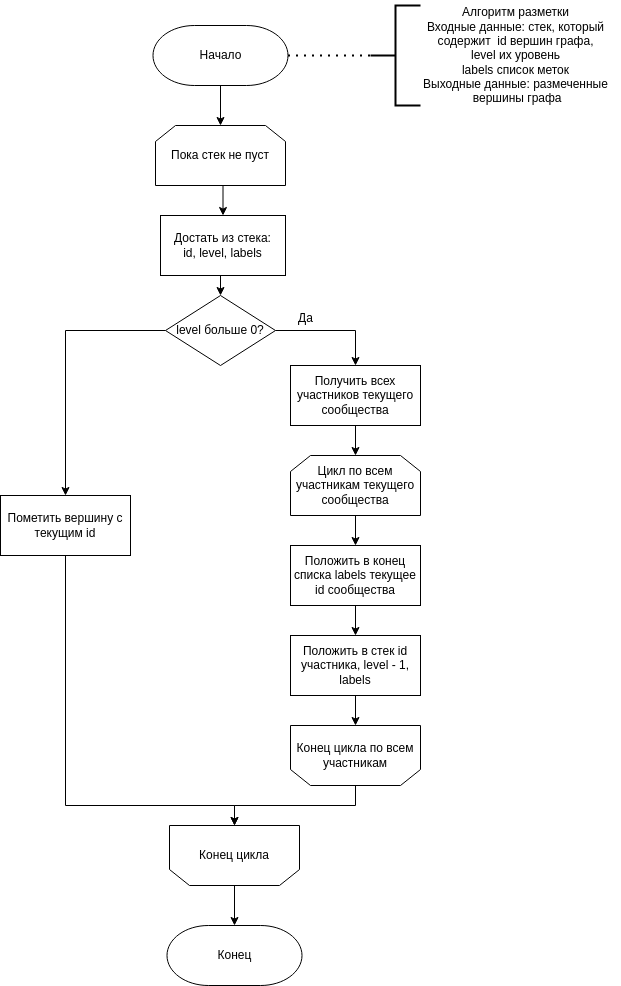
\includegraphics[height=0.6\textheight]{Tag alg.png}
	\caption{Схема алгоритма разметки пользователей социальной сети по сообществам}
	\label{fig:tag alg}
\end{figure}

\section*{Вывод}

В рамках конструкторской части были выделены основные сущности и отношения предметной области, отражающие структуру социальной сети и её сообществ. На основании этого была спроектирована база данных, ориентированная на хранение и обработку графовых данных.

Также был разработан алгоритм разметки пользователей по сообществам, учитывающий иерархическую структуру. Использование обхода в глубину (DFS) с явным стеком обеспечивает корректную работу с глубокими уровнями вложенности и позволяет эффективно сопоставлять каждому пользователю все уровни его принадлежности. Предложенная структура и методы обеспечивают надёжную основу для дальнейшей обработки и анализа социальной графовой модели.
